\section{HIMA Hardware (H51q-HS)}
The first part of lab was to become more familiar with the HIMA 
Programmable Electronic System (PES) hardware. The purpose of such systems is to increase safety in industrial processes. As well to an overall reduction of the system price, engineering costs, maintenance and commissioning costs. 



\subsection{What is HIMA PES}
The HIMA PES mainly consists of the H41q and H51q system families.
Both system families are based on the same hardware and software, and
they are the 3rd generation of the field-proven HIMA PES to control preferably process engineering plants.

\subsection{What is Planar4} 
Planar4 is the only safety system in the world which can be used up to SIL4 in accordance with IEC 61508. Planar4 is the system of choice for automation processes involving extremely high risks to people, machines and the environment 


\begin{figure}[!htb]
    \centering
    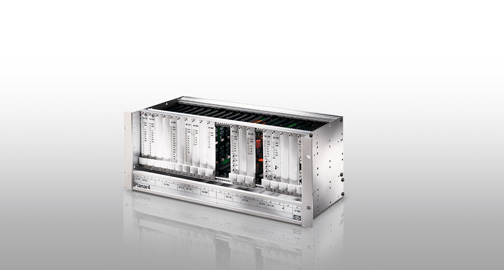
\includegraphics[width=0.8\textwidth]{images/Planar4}
     \caption{Planar4 System}
\end{figure}


